%\documentclass[fleqn, letterpaper]{amsart}
\documentclass[fleqn, letterpaper]{tufte-handout}
\usepackage{times}
\usepackage{amsmath}
\usepackage{amssymb}
\usepackage{graphicx}
\usepackage{booktabs}
\usepackage{multirow}
\usepackage{listings}
\usepackage{epstopdf}
\usepackage{bm}
\usepackage{natbib}
%\usepackage[left=1in]{geometry}

\newcommand{\R}{\mathcal{R}}
\newcommand{\E}{\text{E}}
\newcommand{\p}{p_{XY}}
\newcommand{\T}{^\text{T}}
\renewcommand{\arraystretch}{1.5}
\renewcommand{\vec}[1]{\mathrm{#1}}

\title{Problem Set 6 --- ENCE689E Spring 2014}
\author{David Prentiss}

\begin{document}
\maketitle

\section{1. Kalman Filter}
\subsection{(a)}
\begin{align*}
        \frac{dy}{dt} &= \phi y_t + \psi + u(t) \\
        \frac{y_{t+1}-y_t}{\Delta t} &= \phi y_t + \psi + u(t) \\
        \frac{y_{t+1}}{\Delta t} &= \phi y_t + \psi + u(t) + y_t\\
                                 &= \begin{pmatrix} \phi_1+1 & \phi_2 \\ \phi_3 &\phi_4+1\end{pmatrix} y_t + \psi + u(t)\\
        y_{t+1} &= Ay_t + b\psi + cu(t),
\end{align*}
where $A = \begin{pmatrix} \phi_1+1 & \phi_2 \\ \phi_3 &\phi_4+1\end{pmatrix}\text{ and } b = c = \Delta t
$.

\subsection{(b)}
\[z = Hy + v\]

\subsection{(c)}
\begin{align*}
        \bar{y}_{t+1}
\end{align*}
where $ H = (1\quad 0)\T $ and $v\sim\mathcal{N}(\bar{v},\ C_{vv})$

\section{2. Kalman Filter}

{\scriptsize
        \begin{minipage}{\linewidth}
                \lstinputlisting[language=Matlab, caption={Propagation of a linear soil moisture model},
                basicstyle=\ttfamily, label=lst1]{ps6.m}
        \end{minipage}
}

\subsection{(a)}
\begin{align*}
\begin{pmatrix}
\mathbf{y}_{t+1} \\
\mathbf{u}_{t+1} \\
\end{pmatrix}
&=
\begin{pmatrix}
a\mathbf{y}_t + \mathbf{u}_t \\
\rho\mathbf{u}^{(true)}_t+ \mathbf{w}_t
\end{pmatrix}
\end{align*}

\subsection{(b)}

\subsection{(c)}
See figures \ref{2ca} and \ref{2cb}.
\begin{figure}
        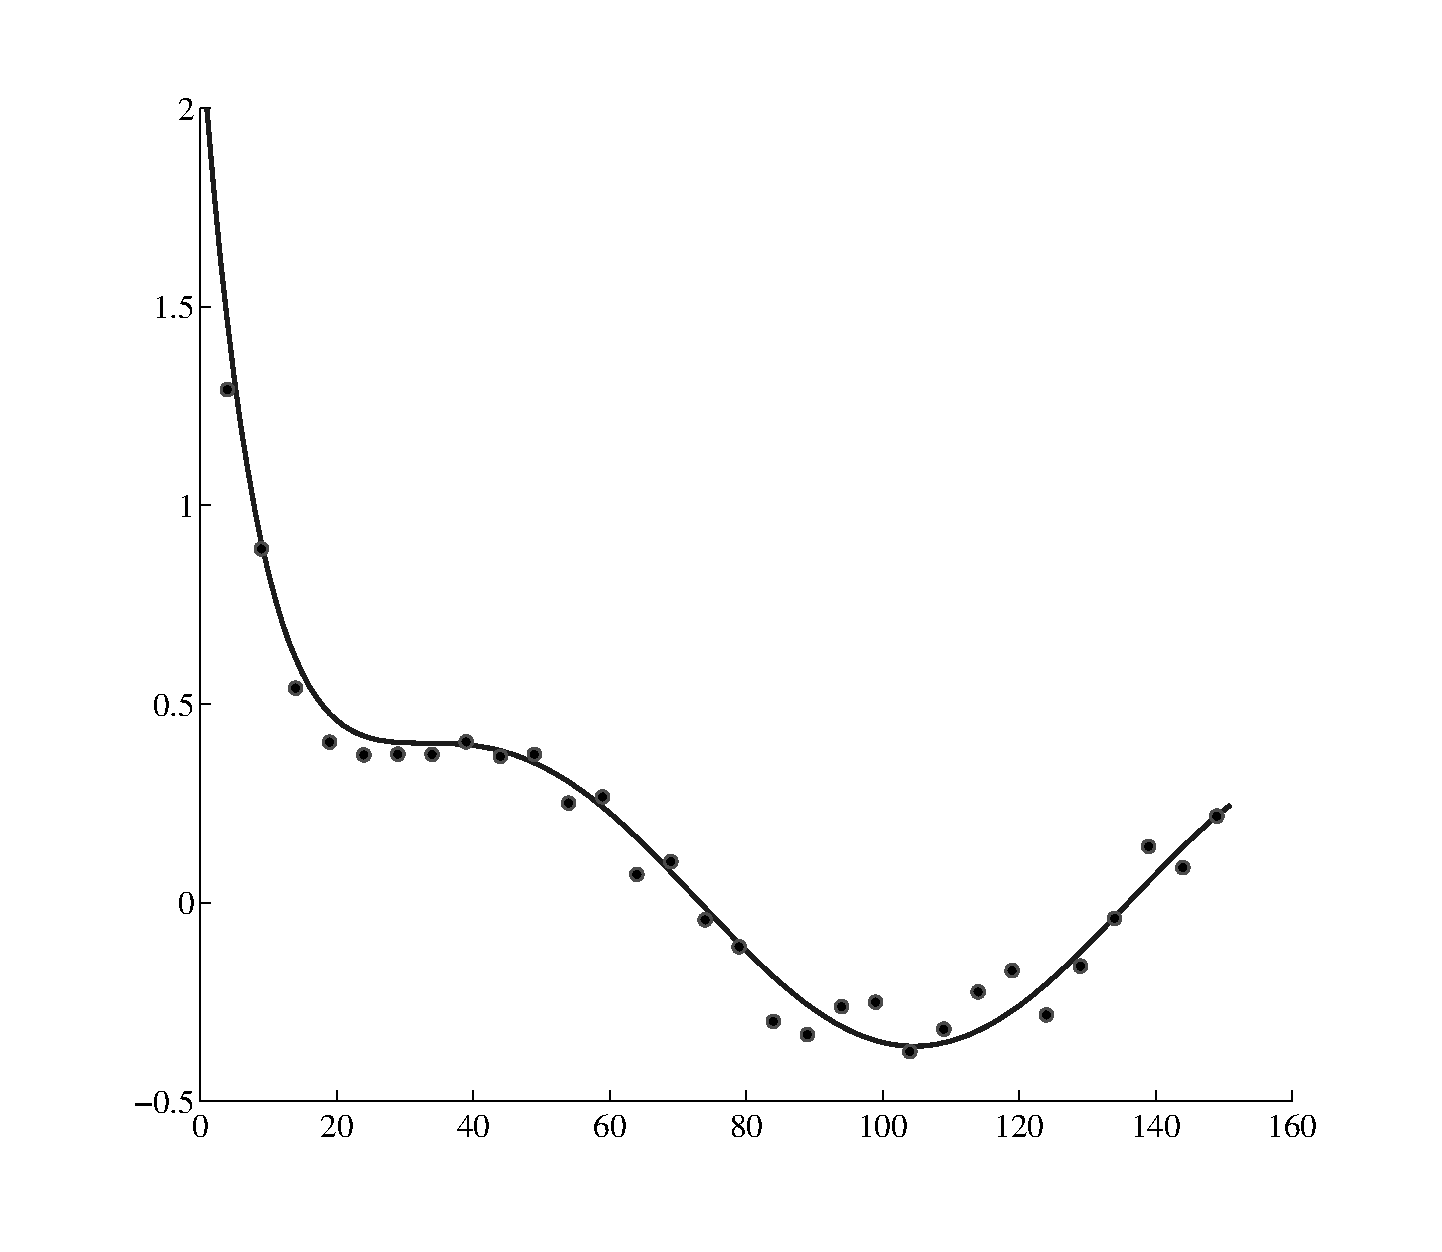
\includegraphics[width=\textwidth]{2ca}
        \caption{True, single-state system and simulated measurement error.}
        \label{2ca}
\end{figure}
\begin{figure}
        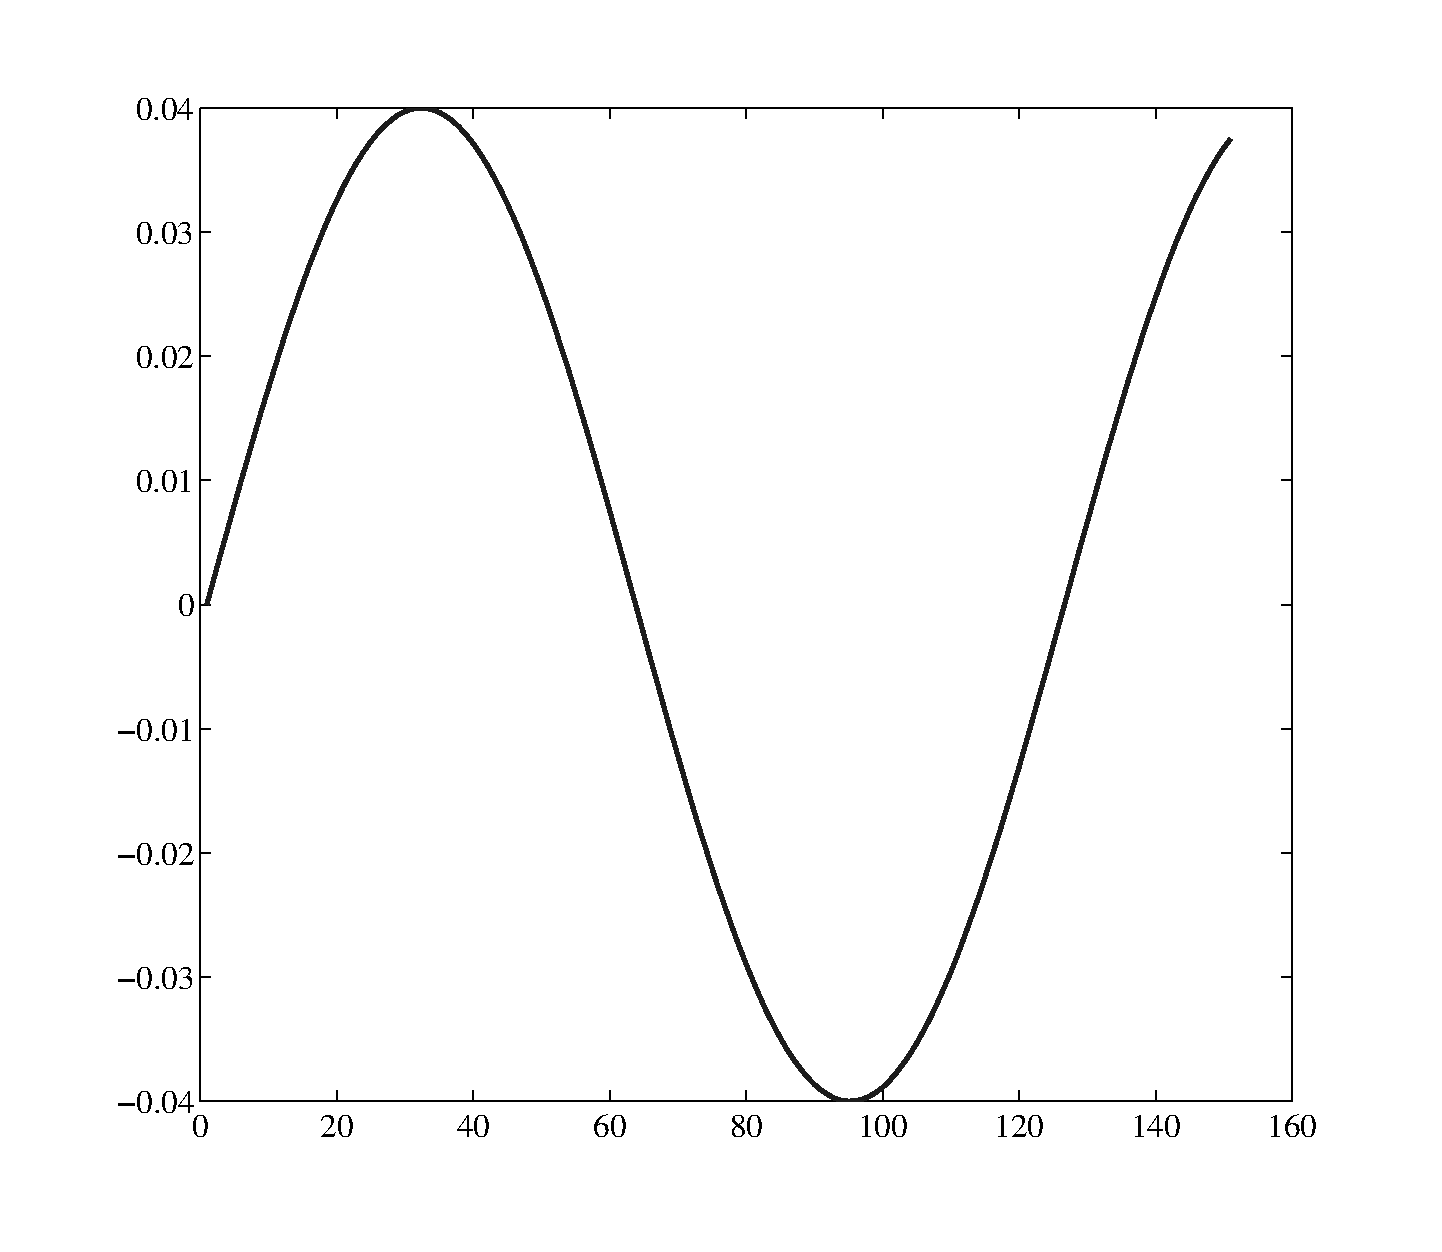
\includegraphics[width=\textwidth]{2cb}
        \caption{True model forcing}
        \label{2cb}
\end{figure}

\subsection{(d)}
\subsection{(e)}
From our samples of \texttt{ytrue} and \texttt{utrue} we can take the sample covariance of each and construct the variavce matrix. Since the errors are uncorrelated, only the diagonals have non-zero values.
\[
\begin{bmatrix} 0.1942 & 0 \\ 0 & 0.0008
\end{bmatrix}
\]
\subsection{(f)}
\begin{figure}
        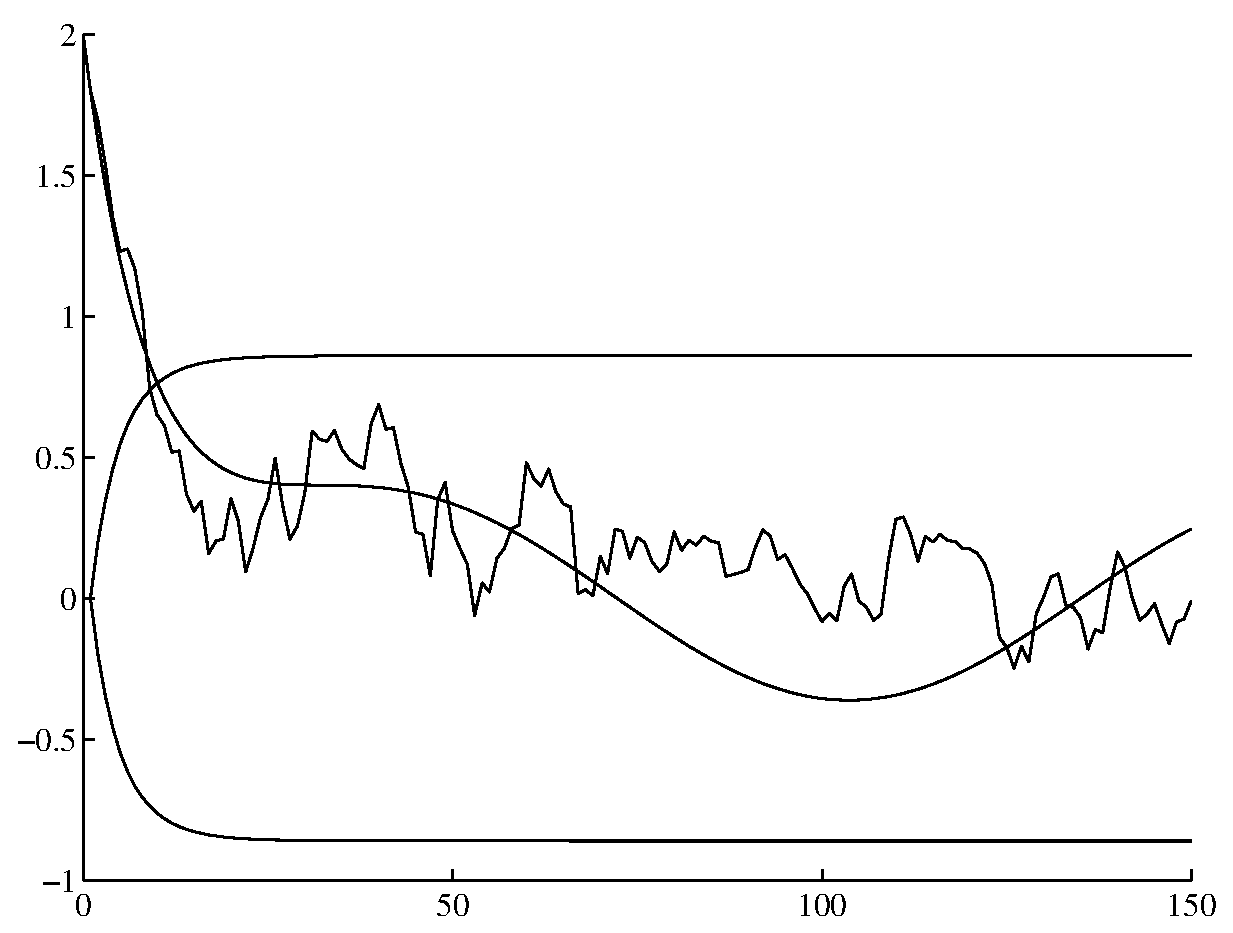
\includegraphics[width=\textwidth]{2fa}
        \caption{True, single-state system and simulated measurement error.}
        \label{2fa}
\end{figure}
\begin{figure}
        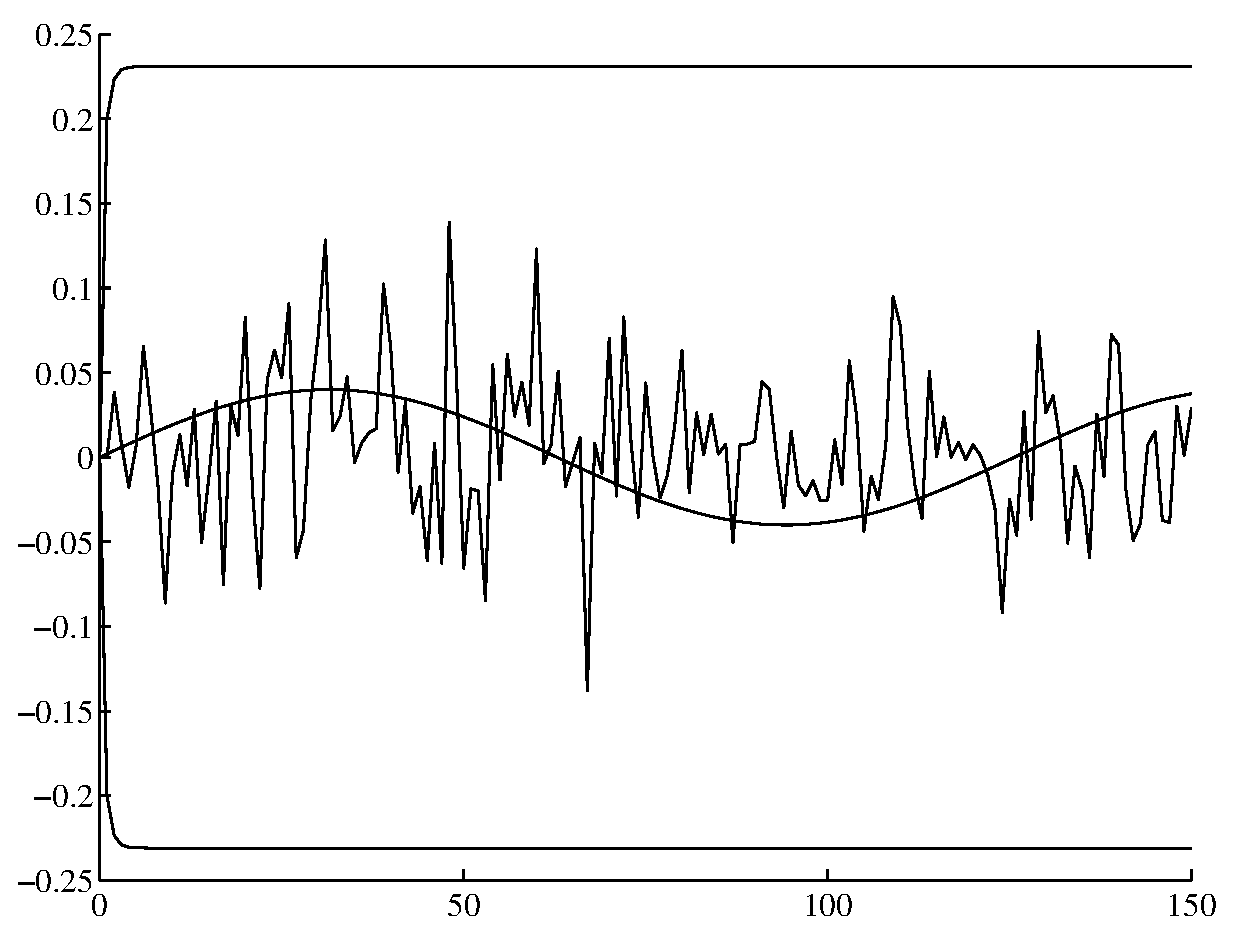
\includegraphics[width=\textwidth]{2fb}
        \caption{True, single-state system and simulated measurement error.}
        \label{2fb}
\end{figure}
{\scriptsize
        \begin{minipage}{\linewidth}
                \lstinputlisting[language=Matlab, caption={Propagation of a linear soil moisture model},
                basicstyle=\ttfamily, label=lst1]{ps6f.m}
        \end{minipage}
}

ans =

   -0.1101


ans =

    0.2727


ans =

   -0.0028


ans =

    0.0506

\subsection{(g)}
{\scriptsize
        \begin{minipage}{\linewidth}
                \lstinputlisting[language=Matlab, caption={Propagation of a linear soil moisture model},
                basicstyle=\ttfamily, label=lst1]{ps6g.m}
        \end{minipage}
}
ans =

    0.0026


ans =

    0.0326


ans =

   3.9219e-04


ans =

    0.0047
\begin{figure}
        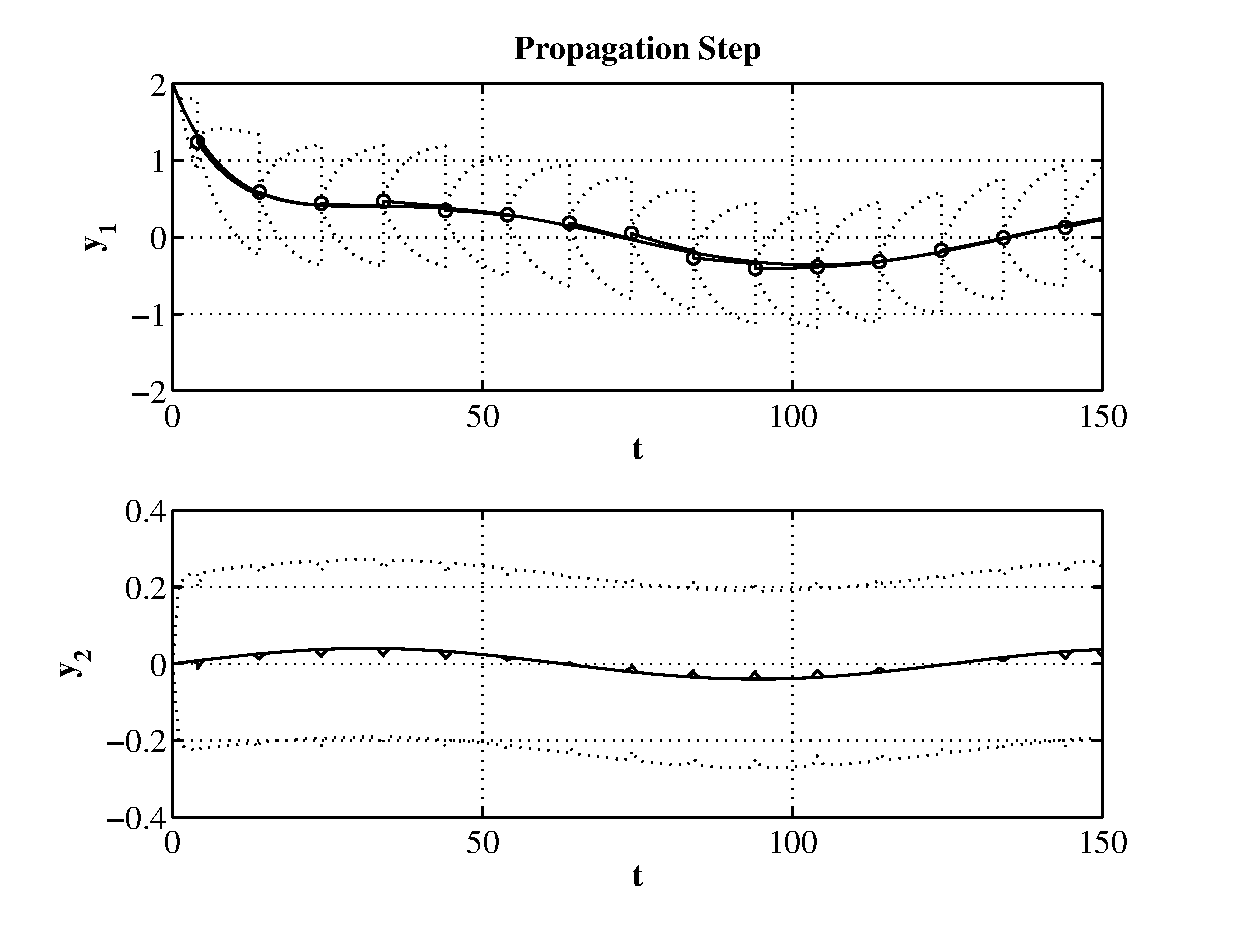
\includegraphics[width=\textwidth]{2g}
        \caption{True, single-state system and simulated measurement error.}
        \label{2g}
\end{figure}
\end{document}
